\EXERCISE
$n \geq 1$
قطاع دایره در شکل زیر را با
$k \geq 3$
رنگ، رنگ‌آمیزی می‌کنیم با این شرط که هر قطاع را با یک رنگ، رنگ می‌کنیم و هر دو قطاع مجاور را با دو رنگ متمایز.
$a_n$
را تعداد راه‌های رنگ‌آمیزی تعریف می‌کنیم.
\begin{center}
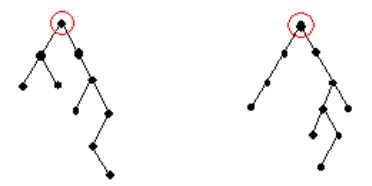
\includegraphics[height=4.5cm]{19.png}
\end{center}
\begin{enumerate}
\item
$a_1, a_2, a_3$
را محاسبه کنید.
\item
یک رابطه‌ی بازگشتی برای
$a_n$
پیدا کرده و آن را حل کنید.
\end{enumerate}